% Simple_UAVCtrl_BlockDiagram.tex
\tikzset{%
  every neuron/.style={
    circle,
    draw,
    minimum size=1cm,
		line width=1.0mm
  },
  neuron missing/.style={
    draw=none, 
    scale=4,
    text height=0.333cm,
    execute at begin node=\color{black}$\vdots$
  },
}

\tikzstyle{ArrowObject1}=[line width=1.5mm, -latex]
\tikzstyle{ArrowObject2}=[line width=1.5mm, latex-]

\resizebox{!}{0.45\textwidth}{
	\begin{tikzpicture}[x=1.5cm, y=1.5cm, >=stealth]
		\draw[help lines,xstep=.5,ystep=.5] (-3,-3) grid (8,4);
		\foreach \x in {-3,-2,...,8} { \node [anchor=north] at (\x/1,0) {0.\x}; }
		\foreach \y in {-3,-2,...,4} { \node [anchor=east] at (0,\y/1) {0.\y}; }
		
		% Input layer nodes
		\foreach \m/\l [count=\y] in {1,2,3}
			\node [every neuron/.try, neuron \m/.try] (input-\m) at (0,2.5-\y) {};
		% Hidden layer nodes
		\foreach \m [count=\y] in {1,2,3,missing,4}
			\node [every neuron/.try, neuron \m/.try ] (hidden-\m) at (3,4.0-\y*1.10) {};
		% Output layer nodes
		\foreach \m [count=\y] in {1,2,missing,3}
			\node [every neuron/.try, neuron \m/.try ] (output-\m) at (6,3.0-\y) {};

		% Input layer labels
		%\foreach \l [count=\i] in {1,2,3}
			\draw [ArrowObject2] (input-1) -- ++(-2.0,0)
				node [above, midway] {Inertial};
			\draw [ArrowObject2] (input-2) -- ++(-2.0,0)
				node [above, midway] {Pressure};
			\draw [ArrowObject2] (input-3) -- ++(-2.0,0)
				node [above, midway] {Strain};
		% Hidden layer labels
		\foreach \l [count=\i] in {1,2,3,n}
			\node [above] at (hidden-\i.north) {$H_\l$};
		% Output layer labels
		%\foreach \l [count=\i] in {1,2,n}
		  \draw [ArrowObject1] (output-1) -- ++(2,0);
			\draw [ArrowObject1] (output-2) -- ++(2,0);
			\draw [ArrowObject1] (output-3) -- ++(2,0);
		  \only<3->{
			  \draw [ArrowObject1] (output-1) -- ++(2,0)
				  node [above, midway] {$\alpha, \,\beta,  \,V$};
			}
			\only<4->{
			  \draw [ArrowObject1] (output-2) -- ++(2,0)
				  node [above, midway] {$C_{L}, \,C_{D}, \,\ldots$};
			}
			\only<7->{
			  \draw [ArrowObject1] (output-3) -- ++(2,0)
				  node [above, midway] {$\delta_{ail}, \,\delta_{ele}, \,\ldots$};
			}
				
		% Input layer connecting arrows
		\foreach \i in {1,...,3}
			\foreach \j in {1,...,4}
				\draw [ArrowObject1] (input-\i) -- (hidden-\j);
		% Hidden layer connecting arrows
		\foreach \i in {1,...,4}
			\foreach \j in {1,...,3}
				\draw [ArrowObject1] (hidden-\i) -- (output-\j);

		\foreach \l [count=\x from 0] in {Input, Hidden, Output}
			\node [align=center, above] at (0,-2.75) {Input\\layer};
			\node [align=center, above] at (3,-2.75) {Hidden\\layers};
			\node [align=center, above] at (6,-2.75) {Output\\layer};

	\end{tikzpicture}
}